\section{Scattering}

Now that we have shown that the qubit state induces a frequency shift on the resonator, it remains to show how we measure that frequency shift.
In this part of the calculation we omit the qubit, taking its effect on the system into account through the resonator frequency shift.
Therefore, this calculation is classical, with the quantum effect of the qubit encapsulated in the parameter $\chi$ calculated in the previous section.

We consider a resonator connected in parallel to a transmission line, as shown in Fig.\,\ref{Fig:scatteringDiagram}.
A resonator with impedance $Z_r$ and frequency $\omega_r$ is connected in parallel through a capacitor $C_{\kappa}$ to a transmission line.
We model the resonator as a parallel LC circuit with resonance frequency $\omega_{LC}=1/\sqrt{LC}$, internal quality factor $Q_i$ and characteristic impedance $Z_{LC}=\sqrt{L/C}$.
The shunt impedance is $Z_{\text{in}}=Z_{\kappa} + Z_r$ where $Z_{\kappa} = 1/i\omega C_{\kappa}$ is the impedance of the coupling capacitor, and $Z_r = Z_{LC}Q_i/(1+iQ_i(x-1/x))$ with $x \equiv \omega/\omega_{LC}$ is the impedance of the resonator.
The shunt circuit interrupts the transmission line, creating a scattering site for traveling microwave signals in the line.
A voltage wave injected into the input port with amplitude $V_{\textrm{in}}$ scatters from the shunt circuit.
Part of the wave reflects with amplitude $V_{\textrm{in}}S_{11}$ and part is transmitted with amplitude $V_{\textrm{out}}=V_{\textrm{in}}S_{21}$.
In the following analysis, we show how, by measuring the amplitude and phase of the scattered signal, we can infer the frequency of the resonator, and thus the state of the qubit.

\begin{figure}
\begin{centering}
\includegraphics[width=9cm]{basic_circuit.pdf} 
\par\end{centering}
\caption{A transmission line shunted by a resonant circuit. In incoming voltage wave is partially reflected and partially transmitted by the impedance mismatch at the point where the resonator is coupled to the transmission line.}
\label{Fig:scatteringDiagram}
\end{figure}

The scattering parameters $S_{ij}$ for a transmission line interrupted by a shunt circuit with admittance $Y=1/Z_{\text{in}}$, as shown in Fig.\,\ref{Fig:scatteringDiagram}, are \cite{Pozar:microwaveEngineering2009} \begin{eqnarray}
S_{11} &=& \frac{-\bar{Y}}{2+\bar{Y}} \label{eq:S11_Y} \\
S_{21} &=& \frac{2}{2+\bar{Y}} \, , \label{eq:S21_Y} \end{eqnarray}
where $\bar{Y} \equiv Z_0 Y$ and $Z_0$ is the characteristic impedance of the transmission line.
From these equations we can solve for $S_{11}$ in terms of $S_{21}$, \begin{equation}
S_{11} = S_{21} - 1 \, . \label{eq:S11S21} \end{equation}

The qubit state measurement is based on the fact that the output voltage wave amplitude depends on the properties, namely $Q$ and $\omega_r$, of the resonator.
To describe this we must compute $S_{21}$ in terms of probe frequency and the resonator parameters.
Using Eq.\,(\ref{eq:S21_Y}) it can be shown that \begin{eqnarray}
S_{21} &=& \frac{S_{\textrm{min}} + 2iQ_l \delta y}{1+2iQ_l \delta y} \label{eq:S21} \\
\Re S_{21} &=& \frac{S_{\textrm{min}}+(2Q_l\delta y)^2}{1+(2Q_l\delta y)^2} \\
\Im S_{21} &=& \frac{2Q_l\delta y(1-S_{\textrm{min}})}{1+(2Q_l\delta y)^2} \, , \end{eqnarray}
where $Q_l^{-1} = Q_i^{-1} + Q_c^{-1}$, $Q_c$ is the coupled $Q$ of the resonator, $S_{\textrm{min}} = Q_c/(Q_c + Q_i)$, and $\delta y \equiv (\omega - \omega_r) / \omega_r$ where $\omega_r$ is the resonance frequency \cite{Mazin:thesis2004}.\footnote{The frequency $\omega_r$ is near to the resonator bare resonance but slightly detuned due to the coupling capacitor and line impedance.}
A result that will be useful later is that the imaginary part of $S_{21}$ is extremal for $\delta y = \pm 1/2Q_l$.

\begin{figure}
\begin{centering}
\includegraphics[width=8cm]{S21_circle.pdf} 
\par\end{centering}
\caption{Scattering diagram for shunt resonator}
\label{Fig:S21Circle}
\end{figure}

The inverse transmission amplitude is a very useful quantity \begin{equation}
S_{21}^{-1} = 1 + e^{i\phi}\frac{Q_i}{Q_c}\frac{1}{1+2i Q_i \delta y} \end{equation}
This equation comes from inverting the usual expression for $S_{21}$ and adding a phase factor in the second term to account for possible impedance mismatches between the input and output \cite{Megrant:highQ2012}. The diameter of the circle is \begin{equation}
D = 1-S_{\textrm{min}}. \end{equation}
Another useful relation is the detuning as a function of the measure transmission amplitude \begin{equation}
\delta x = \frac{1}{2iQ_i}\left[ e^{i\phi} \frac{Q_i}{Q_c} \left(S_{21}^{-1} - 1 \right)^{-1} - 1 \right]. \end{equation}
